\cleardoublepage
\section{Thiết kế mạch schmitt-trigger với $V_{low-threshold} = 1V$, $V_{high-threshold} = 4V$, $V_{ref} = 5V$, $V_{out} = 5V$, và kiểm tra lại bằng proteus}
\begin{figure}[H]
    \centering
    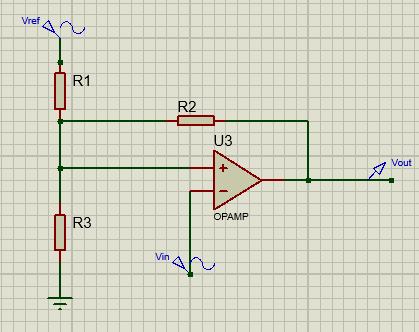
\includegraphics[width=0.7\textwidth]{pictures/smith}
    \caption{Mạch schmitt-trigger}
\end{figure}
    \subsection{Khi $V_{out} = 0V$}
Ta có sơ đồ đấu nối như sau:
\begin{figure}[H]
    \centering
    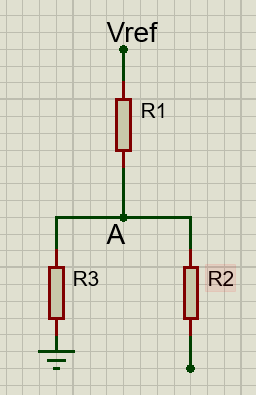
\includegraphics[width=0.35\textwidth]{pictures/Vo_0.png}
    \caption{Khi $V_{out} = 0V$}
\end{figure}
\begin{itemize}
    \item Gọi $V_{A1}$ là điện áp của nút A khi $V_{out} = 0V$.
    \item Khi đó ta có $V_{A1} = \frac{R_{23}}{R_1+R_{23}}V_{ref} = V_{low-threshold}$.
\end{itemize}
\subsection{Khi $V_{out} = 5V$}
Ta có sơ đồ đấu nối như sau:
\begin{figure}[H]
    \centering
    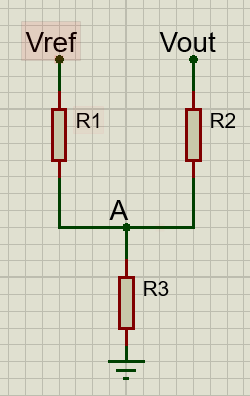
\includegraphics[width=0.35\textwidth]{pictures/Vo_5.png}
    \caption{Khi $V_{out} = 5V$}
\end{figure}
\begin{itemize}
    \item Gọi $V_{A2}$ là điện áp của nút A khi $V_{out} = 5V$.
    \item Khi đó ta có $V_{A2} = \frac{R_3}{R_1+R_{12}}V_{ref} = V_{high-threshold}$.
\end{itemize}
    \subsection{Thiết kế mạch Schmitt-Trigger}
Gọi $R_1 = x$, $R_2 = y$, $R_3 = z$.
Ta có hệ sau:
\begin{align}
\frac{yz}{xz+yz+zy} = \frac{y}{x+2y} = \frac{V_{A1}}{V_{ref}} = \frac{V_{low-threshold}}{V_{ref}} = \frac{1}{5} 
    \rightarrow x = 3y \\
    \frac{xz+zy}{xz+yz+xy} = \frac{V_{A2}}{V_{ref}} = \frac{V_{high-threshold}}{V_{ref}} = \frac{4}{5}
\end{align}
Thay (3) vào (4) ta được:
\[
\frac{4yz}{4yz + y^2} = \frac{4z}{4z+y} = \frac{4}{5} \Rightarrow y = z
\]
Chọn x = $R_1$ = 60k$\Omega$, y = z = $R_2 = R_3 =$ 20k$\Omega$.\\
\begin{figure}[H]
    \centering
    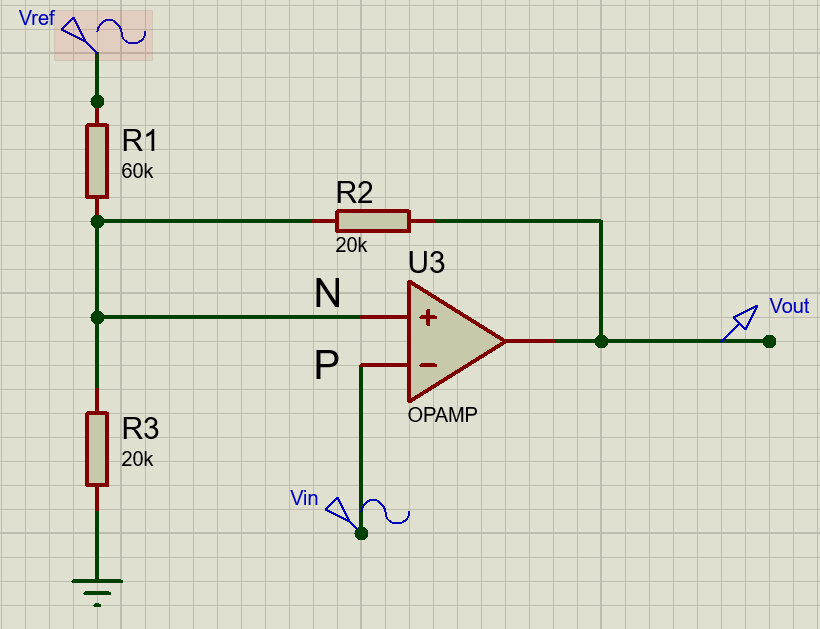
\includegraphics[width=0.7\textwidth]{pictures/smith2}
    \caption{Mạch schmitt-trigger sau khi tính toán các giá trị điện trở}
\end{figure}
\subsection{Tìm mối quan hệ giữa $V_{out}$ và $V_{in}$}
\hspace*{0.6cm}\textbf{Giả sử KĐTT là lý tưởng}
				\[
				\Rightarrow
				\begin{cases}
					I^+ = I^- = 0\\
					V_N = V_P\\
				\end{cases}
				\]
Áp dụng định luật Kifhoff tại nút P:
\begin{align}
    V_p = V_{in}
\end{align}
Áp dụng định luật Kifhoff tại nút N:
\[
    \frac{V_N-V_{ref}}{60} + \frac{V_N}{20} + \frac{V_N-V_{out}}{20} = 0 \\ 
\]
\[
    \Longleftrightarrow V_N - V_{ref} + 6V_N - 3V_{out} = 0 
\]
\[
    \Longleftrightarrow 7V_{in} - V_{ref} = V_{out}
\]
Với $V_{in} = 5sin(100\pi t)$, $V_{ref} = 4sin(100/pi t)$.
\[
    \Rightarrow V_{out} = \frac{7 \cdot 5sin(100\pi t) - 4sin(100\pi t)}{3}
\]
\begin{align}
    \Rightarrow V_{out} = 10.333sin(100\pi t)
\end{align}
\cleardoublepage
\subsection{Kiểm tra lại bằng proteus}
\hspace*{0.6cm}Sau khi nhập các giá trị $V_{in} = 5V$, $V_{ref} = 4V$ với tần số 50Hz vào mạch schmitt-trigger, ta thu được kết quả như sau:
\begin{figure}[H]
    \centering
    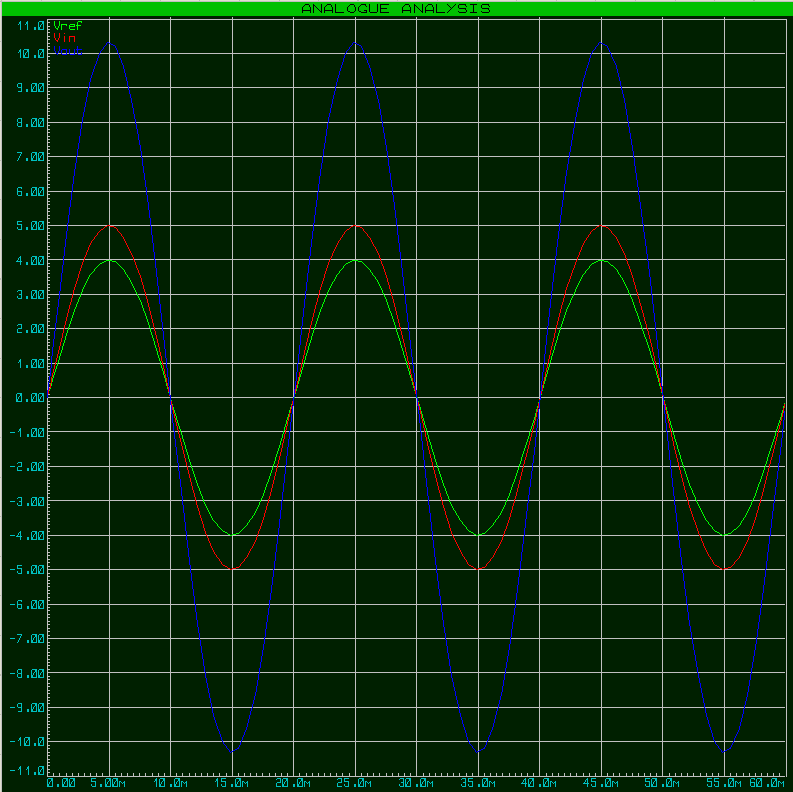
\includegraphics[width=1\textwidth]{pictures/smithplot}
    \caption{Kết quả mô phỏng mạch schmitt-trigger}
\end{figure}
Căn cứ vào đồ thị ta thấy giá trị điện áp đầu ra có biên độ = 10.333 và pha ban đầu giống với $V_{out} = 10.333sin(100\pi  t)$ đã tìm được ở trên\\
\hspace*{0.6cm}$\Rightarrow$ \textbf{Kết quả mô phỏng proteus giống với giá trị tính toán.}